
\begin{figure}[H]
    \centering
    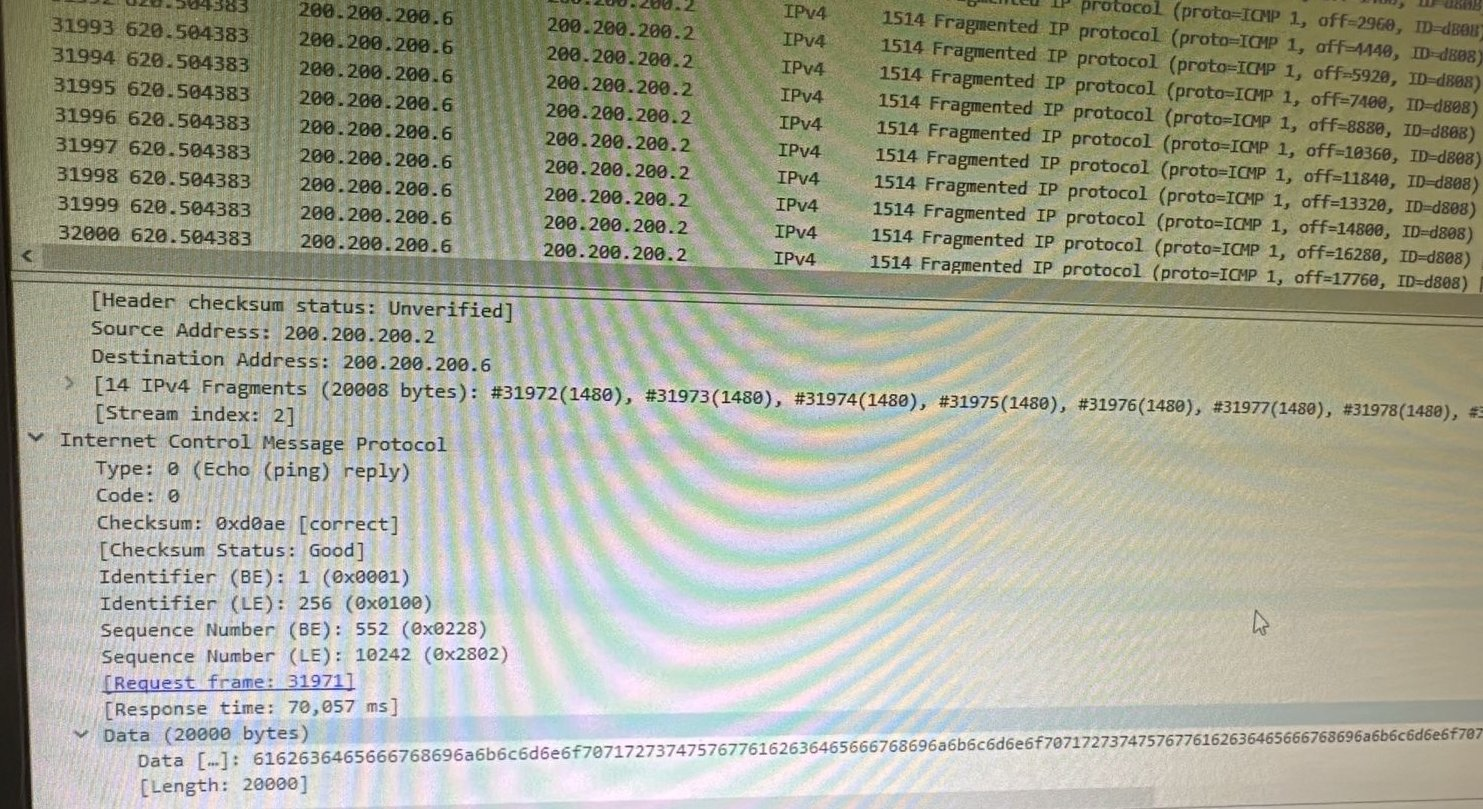
\includegraphics[width=\columnwidth]{punto1/p1_ws_wifi_lan_20k.jpeg}
    \caption{Wireshark Wifi - Lan, 20000}
    \label{fig:ws_wifi_lan_20k}
\end{figure}

\begin{figure}[H]
    \centering
    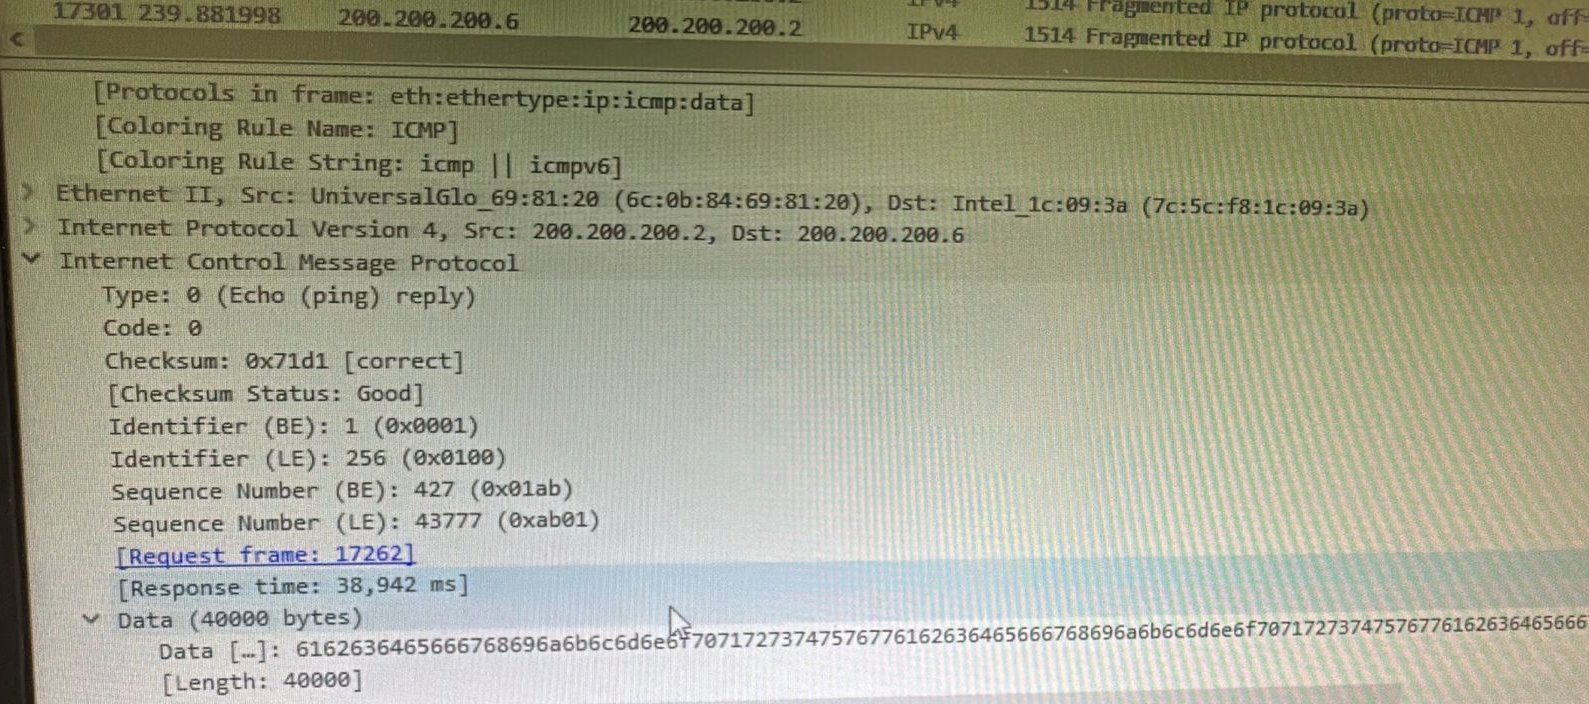
\includegraphics[width=\columnwidth]{punto1/p1_ws_wifi_lan_40k.jpeg}
    \caption{Wireshark Wifi - Lan, 40000}
    \label{fig:ws_wifi_lan_40k}
\end{figure}

\begin{figure}[H]
    \centering
    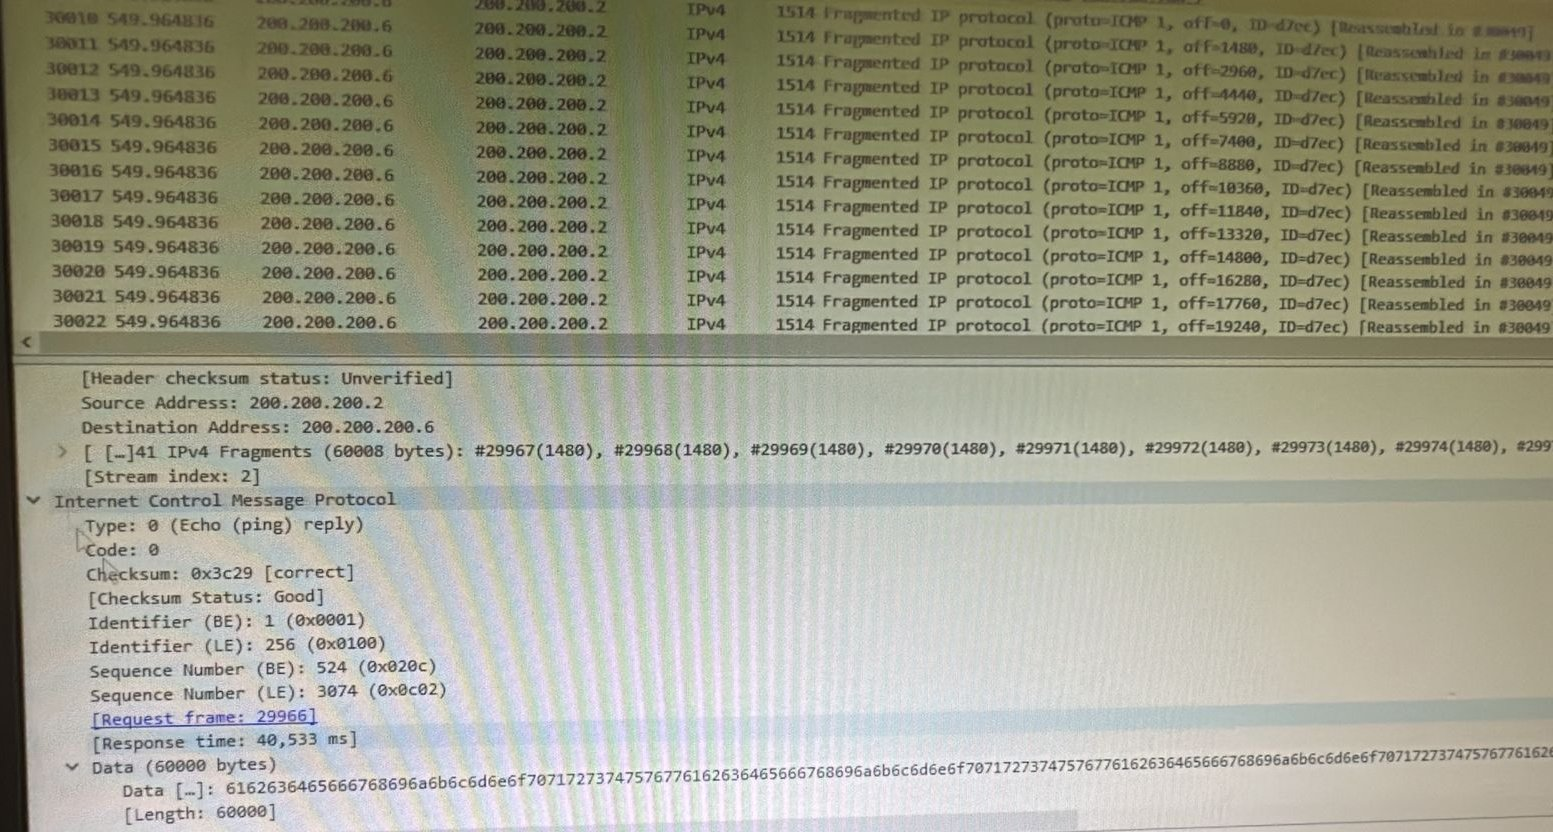
\includegraphics[width=\columnwidth]{punto1/p1_ws_wifi_lan_60k.jpeg}
    \caption{Wireshark Wifi - Lan, 60000}
    \label{fig:ws_wifi_lan_6k}
\end{figure}

\subsection{Montaje}

%Explique:
% Encabezado IPv4. Explicar de acuerdo al montaje (instalación) realizada en la parte 1 los valores obtenidos.
% Campos de ICMP (Echo Request / Echo Reply). Cuando ejecuto los pings.
% Tiempos de ida y vuelta (RTT). Cuando ejecuto los pings.
% Compare velocidades teóricas vs. Prácticas, cambiando el tamaño del ping

\subsection{Aplicación IA}
Se exportar la captura. pcap y usar una herramienta de IA que explique lospatrones de tráfico, anomalías y latencias.
